
\documentclass[a4paper,14pt]{extarticle}
\usepackage{cmap}
\usepackage[T2A]{fontenc}
\usepackage[utf8]{inputenc}
\usepackage{setspace}
\usepackage{titlesec}
\usepackage{diagbox}
%\renewcommand{\baselinestretch}{1.5}
\onehalfspacing
\usepackage[english,russian]{babel}
\usepackage{comment}
\usepackage{amsmath,amsfonts,amssymb,mathtext,cite,enumerate,float,indentfirst,floatflt}

\usepackage[left=3cm,right=1cm,
    top=2cm,bottom=2cm,bindingoffset=0cm]{geometry}
		
\renewcommand{\refname}{whatever}	
		
\usepackage{multicol,subcaption,multirow}
\usepackage{graphicx,caption,tocvsec2}

\addto\captionsrussian{\def\refname{СПИСОК ИСПОЛЬЗОВАННЫХ ИСТОЧНИКОВ}}

\usepackage{fancyhdr,fancybox}
\graphicspath{{images_errors_CS/}{images_additional/}{images_errors_EL/}}
\pagestyle{plain}
\fancyhead[L]{\thepage}
\renewcommand{\headrulewidth}{0pt}

\captionsetup[subfigure]{labelformat=simple, labelsep=colon}
\renewcommand{\thesubfigure}{\alph{subfigure}}

\titleformat*{\section}{\large\bfseries}
\titleformat*{\subsection}{\normalsize\bfseries}

\makeatletter
\renewcommand*{\@alph}[1]{%
  \ifcase#1\or а\or б\or в\or г\or
    д\or е\or ё\or ж\or з\or и\or й\or
    к\or л\or м\or н\or о\or п\or р\or с\or\v т\or
    у\or ф\or х\or ц\or ч\or ш\or щ\or ъ\or ы\or ь\or э\or ю\or \v я\else\@ctrerr\fi
}
\makeatother

\begin{document}

\begin{comment}
\begin{center}
\section*{\centering РЕФЕРАТ}
\end{center}
\setcounter{page}{2}
\addcontentsline{toc}{section}{РЕФЕРАТ}

Расчётно-пояснительная записка 63 с., 20 рис., 27 табл., 15 источников.

НАГРУЖЕНИЕ ТРУБЫ, СТАНДАРТНЫЙ МЕТОД КОНЕЧНЫХ ЭЛЕМЕНТОВ, СМЕШАННЫЙ МЕТОД КОНЕЧНЫХ ЭЛЕМЕНТОВ, ДАВЛЕНИЕ, ДЕФОРМАЦИЯ ПОЛЗУЧЕСТИ, СЛАБОСЖИМАЕМЫЙ МАТЕРИАЛ, СХЕМА ЭЙЛЕРА

В технике при рассмотрении задач, связанных с удержанием высокого давления, часто приходится сталкиваться с толстостенными трубами. Определение напряжений в подобной трубе значительно тяжелее, чем в тонкостенных трубах. Вопросы, касающиеся эффективного решения подобных задач относительно разных факторов являются актуальными. 

Цель работы - сравнение численных решений задачи нагружения трубы давлением, полученных с использованием стандартного и смешанного методов конечных элементов, в упругой постановке и в постановке с учётом деформации ползучести.

Результаты, полученные для краевой задачи упругости, показали, что для слабосжимаемого материала правильнее использовать смешанный метод конечных элементов, так как ошибки в вычислении напряжений при решении стандартным методом конечных элементов существенно возрастают, в то время как смешанный метод конечных элементов обладает стабильной точностью. Результаты, полученные для краевой задачи с учётом деформации ползучести, показали, что смешанный метод конечных элементов эффективнее стандартного метода конечных элементов, так как с течением времени аналитическое и численное решения начинают расходиться. 

\newpage

\renewcommand*\contentsname{\begin{center}СОДЕРЖАНИЕ\end{center}}
	
\tableofcontents


\newpage
\begin{center}
\section*{\centering ВВЕДЕНИЕ}
\end{center}
\addcontentsline{toc}{section}{ВВЕДЕНИЕ}

В технике при рассмотрении задач, связанных с удержанием высокого давления, часто приходится сталкиваться с толстостенными трубами. Определение напряжений в подобной трубе значительно тяжелее, чем в тонкостенных трубах. Вопросы, касающиеся эффективного решения подобных задач относительно разных факторов являются актуальными. 

В качестве метода численного решения соответствующей задачи в одномерном приближении (всё зависит только от радиуса) можно применить стандартный метод конечных элементов с использованием линейных базисных функций, но данный способ обладает рядом недостатков при решении задачи упругости для несжимаемого или слабосжимаемого материала. Смешанный метод конечных элементов является эффективным инструментом решения данной проблемы. 

При оценке долговечности и надежности конструкции необходимо учитывать деформации ползучести для корректного определения напряжений. При решении методом конечных элементов краевой задачи с учётом деформации ползучести чаще всего используют простую и экономичную явную схему Эйлера.

Целью работы является сравнение численных решений задачи нагружения трубы давлением, полученных с использованием стандартного и смешанного методов конечных элементов, в упругой постановке и в постановке с учётом деформации ползучести.

Для достижения поставленной цели решены следующие задачи:
\begin{itemize}
\item[-]рассмотрение модели упругого материала и модели материала, учитывающую деформации ползучести;
\item[-]исследование основных соотношений стандартного и смешанного методов конечных элементов для численного решения задачи упругости;
\item[-]реализация смешанного и стандартного методов конечных элементов в виде программы для моделей упругого материала и материала с учётом деформации ползучести;
\item[-]проведение серии расчётов для задачи нагружения упругой трубы давлением;
\item[-]сравнение численных результатов, полученных с помощью смешанного и стандартного методов конечных элементов с аналитическим решением при разных коэффициентах Пуассона для задачи упругости;
\item[-]проведение серии расчётов для задачи нагружения давлением трубы с учётом деформации ползучести;
\item[-]сравнительный анализ численных результатов, полученных с помощью смешанного и стандартного методов конечных элементов, с аналитическим решением задачи установившейся ползучести;
\end{itemize}

\newpage
\section{Математическая модель}
\subsection{Постановка задачи механики твёрдого деформируемого тела}

Для решения общей задачи по определению напряжений и деформаций в деформируемом теле необходимо использовать следующие уравнения равновесия $\left[1\right]$ (считаем, что объёмные силы на тело не действуют):
\begin{equation}\label{EquationEquilGeneral}
\frac{\partial \sigma_{ji}}{\partial x_{j}}=0
\end{equation}
с кинематическим условием на части границы $S_{1}$
\begin{equation}
u=u_{0}
\end{equation}
и с силовым условием на части границе $S_{2}$
\begin{equation*}
\sigma_{ji} n_{j}=p_{i},
\end{equation*}
где $\sigma_{ji}$-компоненты тензора напряжений, $p_i$-компоненты вектора поверхностных сил, $x_{j}$-декартовы координаты. 
 
В общем случае напряжения и деформации описываются тензорами второго ранга в трёхмерном пространстве. Закон Гука выглядит следующим образом:
\begin{equation}\label{GukGeneral}
\sigma_{ij}=C_{ijkl}\varepsilon^{e}_{kl},
\end{equation}
где $C_{ijkl}$-компоненты тензора упругих коэффициентов, $\varepsilon^{e}_{kl}$-компоненты тензора упругих деформаций.
	
Компоненты тензора полных деформаций задаются соотношениями Коши [5]:
\begin{equation}\label{KoshiGeneral}
\varepsilon_{kl}=\frac{1}{2}(\frac{\partial u_k}{\partial x_l}+\frac{\partial u_l}{\partial x_k}),
\end{equation}
где $u_i=u_i(\mathbf{x},t)$-компоненты вектора перемещений.

Для исследования труб удобнее использовать цилиндрическую систему координат. Уравнения равновесия в цилиндрической системе координат записываются в виде [3]
\begin{equation} \label{CSK}
\begin{cases}
\dfrac{\partial \sigma_{rr}}{\partial r}+\dfrac{1}{r}\dfrac{\partial \sigma_{r\varphi}}{\partial \varphi}+\dfrac{\partial \sigma_{zr}}{\partial z}+\dfrac{\sigma_{rr}-\sigma_{\varphi\varphi}}{r}=0 \\
\dfrac{\partial \sigma_{r\varphi}}{\partial r}+\dfrac{1}{r}\dfrac{\partial \sigma_{\varphi\varphi}}{\partial \varphi}+\dfrac{\partial \sigma_{\varphi z}}{\partial z}+\dfrac{2\sigma_{r\varphi}}{r}=0 \\
\dfrac{\partial \sigma_{rz}}{\partial r}+\dfrac{1}{r}\dfrac{\partial \sigma_{\varphi z}}{\partial \varphi}+\dfrac{\partial \sigma_{zz}}{\partial z}+\dfrac{\sigma_{rz}}{r}=0
\end{cases}
\end{equation}

\begin{figure}[ht]
\begin{center}
\includegraphics[width=45mm]{PostZ.png}
\caption{Труба под внутренним и внешним давлением}	
\label{PostZ}
\end{center}
\end{figure}

Длину трубы предполагаем достаточно большой для того, чтобы можно было считать, что осевое напряжение распределено по осевому сечению равномерно, и что удерживающее влияние днищ на радиальные перемещения цилиндра пренебрежимо мало. Будем считать, что в рассматриваемом теле выполнены следующие допущения: все переменные не зависят от координат $\varphi$ и $z$.Таким образом задача по сути сводится к одномерному случаю (всё зависит только от $r$) и уравнения равновесия \eqref{CSK} сводятся к одному уравнению
\begin{equation}\label{EquationEquilGeneralR}
\frac{d}{d\:r}(\sigma_{rr}\: r)-\sigma_{\varphi\varphi}=0
\end{equation}

Данное уравнение \eqref{EquationEquilGeneralR} можно получить не только из общего вида уравнения равновесия, но и другим способом. Рассмотрим полый цилиндр с внутренним радиусом $a$, и наружным $b$, находящийся под действием внутреннего давления $p_a$ и наружного $p_b$. В следствии осевой симметрии цилиндра и нагрузок напряжения и деформации также симметричны относительно его оси. Двумя сечениями, перпендикулярными к оси цилиндра и находящимися друг от друга на расстоянии, равном единице, вырежем кольцо.

В этом кольце выделим элемент двумя плоскостями, проходящими через ось цилиндра и образующими между собой угол $d\varphi$, и двумя соосными цилиндрическими поверхностями с радиусами $r$ и $r+dr$. Нормальные напряжения на цилиндрической поверхности элемента, имеющей радиус $r$ (радиальные напряжения), обозначим через $\sigma_r$; на радиусе $r+dr$ напряжения получат приращения и будут равны $\sigma_r +d\sigma_r$. Нормальные напряжения на плоских гранях (окружные напряжения) обозначим через $\sigma_{\varphi}$.

Вследствие осевой симметрии цилиндра и нагрузок перекашиваться элемент не будет и касательных напряжений на его гранях не возникнет. Поэтому нормальные напряжения $\sigma_r$ и $\sigma_{\varphi}$ будут главными напряжениями. 

Умножая напряжения на площади граней, получим действующие на элемент усилия ($\textbf{F}_i$):
\begin{itemize}
\item[-]$\sigma_r r d\varphi$ - на внутренней цилиндрической грани;
\item[-]$(\sigma_r\: + d\sigma_r)(r+dr)d\varphi$-на наружной цилиндрической грани;
\item[-]$\sigma_{\varphi}dr$-на боковых гранях.
\end{itemize}

\begin{figure}[ht]
\begin{center}
\includegraphics[scale=1.5]{image017.jpg}
\caption{Действующие на элемент трубы усилия}
\end{center}
\end{figure}

\newpage

Так как все силы лежат в одной плоскости и их можно отнести к одной точке, то для равновесия элемента суммы проекций сил на две перпендикулярные оси должны быть равны нулю. Условиями равновесия будут уравнения:
\[
\sum\limits_i {F_{xi}}=0, \ \  \sum\limits_i {F_{yi}}=0.
\]

Благодаря симметрии элемента задачу определения напряжений и перемещений в теле вращения можно решить в функции только одного независимого переменного-радиуса $r$. После подстановки необходимых выражений получим 
\[
-\sigma_{r}r\;d\varphi+(\sigma_{r}+d\sigma_r)(r+dr)\;d\varphi-2(\sigma_{\varphi}dr\;\text{sin}\frac{d\varphi}{2})=0
\]

В силу малости угла $\dfrac{d\varphi}{2}$ принимаем, что sin$\dfrac{d\varphi}{2}=\dfrac{d\varphi}{2}$. После раскрытия всех скобок, сокращения подобных слагаемых и отбрасывания члена высшего порядка малости $d\sigma_{r}\:dr\:d\varphi$ получим дифференциальное уравнение равновесия, совпадающее с \eqref{EquationEquilGeneralR}.

\newpage

\subsection{Модели материала}

\subsubsection{Математическая модель упругого тела}

Для упругого тела упругие деформации совпадают с полными, поэтому закон Гука можно переписать следующим образом:
\begin{equation}\label{GukElastic}
\sigma_{ij}=C_{ijkl}\varepsilon_{kl}.
\end{equation}

Для изотропного тела с учётом принятых допущений компоненты тензоров напряжений и деформаций принимают вид [1]:
\begin{equation}
\sigma_{rr}=(\lambda+2\mu)\varepsilon_{rr}+\lambda\varepsilon_{\varphi\varphi},
\end{equation}	
\begin{equation}
\sigma_{\varphi\varphi}=(\lambda+2\mu)\varepsilon_{\varphi\varphi}+\lambda\varepsilon_{rr},
\end{equation}
\begin{equation}
\sigma_{zz}=\dfrac{\lambda}{2(\lambda+\mu)}(\varepsilon_{rr}+\varepsilon_{\varphi\varphi}),
\end{equation}
\begin{equation}\label{ElEr}
\varepsilon_{rr}=\frac{du}{dr}, 
\end{equation}
\begin{equation}\label{ElEt}
\varepsilon_{\varphi\varphi}=\frac{u}{r},
\end{equation}
\begin{equation}\label{ElEz}
\varepsilon_{zz}=0,
\end{equation}
где $\lambda$, $\mu$-параметры Ламе. 

\newpage

\subsubsection{Математическая модель материала с учётом деформации ползучести}

Предполагаем аддитивное разложение тензора полной деформации на \\ упругую и неупругую составляющие:
\begin{equation}
\varepsilon_{ij}=\varepsilon_{ij}^{e}+\varepsilon_{ij}^{c},
\end{equation}
где $\varepsilon_{ij}^{c}$-компоненты тензора деформации ползучести.

Тогда закон Гука можно записать следующим образом:
\begin{equation}\label{GukCS}
\sigma_{ij}=C_{ijkl}(\varepsilon_{kl}-\varepsilon^{c}_{kl}),
\end{equation}

Для изотропного тела компоненты тензора напряжений в цилиндрической системе координат задаются формулами
\begin{equation*}
\sigma_{rr}=(\lambda+2\mu)(\varepsilon_{rr}-\varepsilon^{c}_{rr})+\lambda(\varepsilon_{\varphi\varphi}-\varepsilon^{c}_{\varphi\varphi}),
\end{equation*}

\begin{equation*}
\sigma_{\varphi\varphi}=(\lambda+2\mu)(\varepsilon_{\varphi\varphi}-\varepsilon_{\varphi\varphi}^{c})+\lambda(\varepsilon_{rr}-\varepsilon_{rr}^{c}),
\end{equation*}

\begin{equation*}
\sigma_{zz}=\dfrac{\lambda}{2(\lambda+\mu)}(\varepsilon_{rr}+\varepsilon_{\varphi\varphi}).
\end{equation*}

Используем теорию течения, согласно которой компоненты скоростей деформации ползучести определяются формулой [9]

\begin{equation}\label{EqStrain}
\dot{\varepsilon}_{ij}^{c}=\tilde{\lambda}\acute{\sigma_{ij}},
\end{equation}
где $\tilde{\lambda}$-некий коэффициент пропорциональности, называемый параметром ползучести, а $\acute{\sigma_{ij}}$-компоненты девиатора тензора напряжений
\begin{equation}
\acute{\sigma_{ij}}=\sigma_{ij}-\frac{1}{3}\sigma_{kk}\delta_{ij}.
\end{equation}

Отметим, что по формуле (\ref{EqStrain}) деформация ползучести является несжимаемой, то есть 
\begin{equation}
\varepsilon_{ii}^{c}=0.
\end{equation}

Введём такие понятия, как интенсивность скорости деформации ползучести [10]
\begin{equation}
\dot{\varepsilon}_{u}^{c}=\sqrt{\dfrac{2}{3}\dot{\varepsilon_{ij}^{c}}\dot{\varepsilon}_{ij}^{c}}
\end{equation}

и интенсивность напряжения [10]

\begin{equation}\label{EffectiveSigma}
\sigma_{u}=\sqrt{\dfrac{3}{2}\acute{\sigma_{ij}}\acute{\sigma_{ij}}}.
\end{equation}

После ряда преобразований формулы (\ref{EqStrain}) получим выражение для неизвестного ранее коэффициента пропорциональности

\begin{equation}
\tilde{\lambda}=\dfrac{3}{2}\dfrac{\dot{\varepsilon}_{u}^{c}}{\sigma_{u}}.
\end{equation}

Будем использовать следующий закон ползучести [9]

\begin{equation}\label{EpsIntCSigmaB}
\dot{\varepsilon_{u}^{c}}=B\sigma_{u}^3,
\end{equation}
где $B$ - функция времени, которая определяется выбором материала. Подставив данное выражение в формулу для коэффициента пропорциональности, получим
\begin{equation}
\tilde{\lambda}=\dfrac{3}{2}B\sigma_{u}^2.
\end{equation}

\newpage

\subsection{Получение аналитических решений}

\subsubsection{Аналитическое решение для задачи упругости}

Рассмотрим цилиндр с внутренним радиусом $a$ и внутренним радиусом $b$. Данный цилиндр одновременно нагружен внутренним давлением $p_a$ и внешним давлением $p_b$. В постановке задачи не учитывается осевая растягивающая сила, поэтому $\sigma_{zz}=0$.

Согласно обобщённому закону Гука, напряжения $\sigma_{rr}$ и $\sigma_{\varphi\varphi}$ связаны с деформациями $\varepsilon_{rr}$ и $\varepsilon_{\varphi\varphi}$ данными выражениями:
\begin{equation}\label{GenGukDef}
\varepsilon_{rr}=\frac{1}{E}\left(\sigma_{rr}-\nu \sigma_{\varphi\varphi}\right); \qquad \varepsilon_{\varphi\varphi}=\frac{1}{E}\left(\sigma_{\varphi\varphi}-\nu \sigma_{\varphi\varphi}\right),
\end{equation}
где $E$-модуль Юнга, $\nu$-коэффициент Пуассона.

Выразим из уравнения окружной деформации (\ref{ElEt}) перемещение $u$ и подставим в уравнение радиальной деформации (\ref{ElEr}):
\begin{equation}\label{ExprDef}
\frac{d}{dr}(\varepsilon_{\varphi\varphi} r)-\varepsilon_{rr}=0.
\end{equation} 

Подставим из (\ref{GenGukDef}) компоненты тензора деформации $\varepsilon_{rr}$ и $\varepsilon_{\varphi\varphi}$ в выражение (\ref{ExprDef}). В таком случае, в дополнение к уравнению равновесия (\ref{EquationEquilGeneralR}) получим соотношение следующего вида [2]:
\begin{equation}\label{EquationEquilGeneralRAlt}
\frac{d}{dr}(\sigma_{\varphi\varphi} r)-\sigma_{rr}=0.
\end{equation}

Складывая и вычитая поочерёдно соотношения (\ref{EquationEquilGeneralR}) и (\ref{EquationEquilGeneralRAlt}), получим два новых выражения:
\begin{equation*}
\frac{d}{dr}\left[(\sigma_{\varphi\varphi}+\sigma_{rr}) r\right]-(\sigma_{\varphi\varphi}+\sigma_{rr})=0;
\end{equation*}
\begin{equation*}
\frac{d}{dr}\left[(\sigma_{\varphi\varphi}-\sigma_{rr}) r\right]+(\sigma_{\varphi\varphi}-\sigma_{rr})=0;
\end{equation*}

Решив данную систему, определяем, что
\begin{equation*}
\sigma_{\varphi\varphi}+\sigma_{rr}=2A; \qquad \sigma_{\varphi\varphi}-\sigma_{rr}=\frac{2B}{r^{2}},
\end{equation*}
где $A$ и $B$ - произвольные постоянные. 

Продолжая преобразования, находим
\begin{equation}\label{SigmaRTAB}
\sigma_{rr}=A-\frac{B}{r^2}, \qquad \sigma_{\varphi\varphi}=A+\frac{B}{r^2}.
\end{equation}

Перемещение $u$ найдём из соотношения для вывода окружной деформации (\ref{ElEt}), используя соотношения (\ref{GenGukDef}) и (\ref{SigmaRTAB}):
\begin{equation}\label{uAB}
u=\frac{2}{E}\left[A(1-\nu)r+B(1+\nu)\frac{1}{r}\right].
\end{equation} 

Теперь из соотношений (\ref{SigmaRTAB}) определим неизвестные произвольные постоянные $A$ и $B$ на основании граничных условий, то есть 
\begin{equation*}
A-\frac{B}{a^2}=-p_a, \qquad A-\frac{B}{b^2}=-p_b,
\end{equation*}
откуда, после преобразований, получаем
\begin{equation*}
A=\frac{p_{a} a^{2}-p_{b} b^2}{b^2 - a^2}, \qquad B=\frac{a^2 b^2}{b^2 -a^2}(p_a -p_b).
\end{equation*}

Подставляя полученные $A$ и $B$ в формулы (\ref{SigmaRTAB}) и (\ref{uAB}), получим итоговые выражения:
\begin{equation}\label{ElasticSigmaRResult}
\sigma_{rr}=\frac{p_a a^2 - p_b b^2}{b^2-a^2}-\frac{a^2 b^2}{r^2}\frac{p_a -p_b}{b^2 -a^2};
\end{equation}
\begin{equation}\label{ElasticSigmaTResult}
\sigma_{\varphi\varphi}=\frac{p_a a^2 - p_b b^2}{b^2-a^2}+\frac{a^2 b^2}{r^2}\frac{p_a -p_b}{b^2 -a^2};
\end{equation}	
\begin{equation}\label{ElasticUResult}
u=\frac{\left(1-2\nu\right)\left(1+\nu\right)}{E}\ \frac{p_a a^2 -p_b b^2}{b^2-a^2}r+\frac{1+\nu}{E}\frac{a^2 b^2}{r}\frac{p_a -p_b}{b^2-a^2};
\end{equation}

\newpage

\subsubsection{Аналитическое решение для задачи с учётом деформации ползучести}
\normalsize
Рассмотрим цилиндр с внутренним радиусом $a$ и внутренним радиусом $b$. Данный цилиндр одновременно нагружен внутренним давлением $p_a$ и внешним давлением $p_b$. Считаем, что осевая деформация ползучести трубы равна нулю: $\varepsilon^{c}_{zz}=0$.

Примем материал изотропным и будем полагать, что изменения объёма в процессе ползучести не происходит и условие несжимаемости  имеет вид:
\begin{equation}\label{Neszhi}
\varepsilon^c_{rr}+\varepsilon^c_{\varphi\varphi}=0.
\end{equation}

В рассматриваемом случае установившейся ползучести [9] пренебрегаем упругой деформацией и считаем, что полная деформация совпадает с деформацией ползучести. Тогда окружная $\varepsilon_{\varphi\varphi}^{c}$ и радиальная $\varepsilon_{rr}^{c}$ деформации ползучести могут быть выражены через радиальное смещение $u^{c}$:
\begin{equation}\label{RadOkrPolz}
\varepsilon_{\varphi\varphi}^{c}=\dfrac{u^{c}}{r}; \ \varepsilon_{rr}^{c}=\dfrac{d u^{c}}{d r}.
\end{equation}

Подставим выражения (\ref{RadOkrPolz}) в условие несжимаемости (\ref{Neszhi}), и в ходе преобразований получим соотношение

\begin{equation}
\dfrac{d u^{c}}{d r}=-\dfrac{u^{c}}{r}.
\end{equation}

Проинтегрировав данное соотношение по радиусу, можно получить уравнение изменения радиального смещения в зависимости от радиуса:
\begin{equation}\label{EquationUC}
u^{c}=\dfrac{C}{r},
\end{equation}
где C-некоторая функция, зависящая от времени. 

Далее, подставив полученное выражение (\ref{EquationUC}) в соотношения окружной и радиальной деформаций ползучести (\ref{RadOkrPolz}), получим
\begin{equation}\label{EquationsEPSCRT}
\varepsilon_{\varphi\varphi}^{c}=\frac{C}{r^2}; \ \varepsilon_{rr}^{c}=-\frac{C}{r^2}.
\end{equation}

Интенсивность деформаций ползучести в поставленной задаче запишем следующим образом:
\begin{equation}\label{IntenDef}
\varepsilon_{u}^{c}=\dfrac{2}{3}\sqrt{(\varepsilon^{c}_{\varphi\varphi})^{2}+\varepsilon_{\varphi\varphi}^{c}\varepsilon_{rr}^{c}+(\varepsilon_{rr}^{c})^{2}}.
\end{equation}

Подставляя в уравнение (\ref{IntenDef}) выражения (\ref{EquationsEPSCRT}), получаем
\begin{equation}\label{EpsIntC}
\varepsilon_{u}^{c}=\frac{2}{\sqrt{3}}\frac{C}{r^2}.
\end{equation}

Основываясь на выражении зависимости компонентов скоростей деформации ползучести от компонентов напряжений
\begin{equation}
\varepsilon^{c}_{ij}=\dfrac{3}{2}\dfrac{\varepsilon_{u}^{c}}{\sigma_{u}}(\sigma_{ij}-\delta_{ij}\sigma_{0}),
\end{equation}
и также учитывая нулевую осевую деформацию, получаем
\begin{equation}\label{ModEqSys}
\left. \begin{array}{c}
\sigma_{\varphi\varphi}-\sigma_{rr}=\dfrac{2}{3}\dfrac{\sigma_{u}}{\varepsilon_{u}^{c}}(\varepsilon_{\varphi}^{c}-\varepsilon_{r}^{c}); \\
\\
\sigma_{zz}-\sigma_{rr}=-\dfrac{2}{3}\dfrac{\sigma_{u}}{\varepsilon_{u}^{c}}\varepsilon_{r}^{c}.
\end{array}\right\}
\end{equation}

Если использовать закон ползучести (\ref{EpsIntCSigmaB}), то преобразовывая выражения (\ref{ModEqSys}) при помощи соотношений (\ref{EquationsEPSCRT}) и (\ref{EpsIntC}), получим
\begin{equation}\label{SystemSigma}
\left. \begin{array}{c} 
\sigma_{\varphi\varphi}-\sigma_{rr}=\bigg(\dfrac{2}{\sqrt{3}}\bigg)^{\tfrac{n+1}{n}} \bigg(\dfrac{C}{B}\bigg)^{\tfrac{1}{n}}\dfrac{1}{r^{2/n}}; \\
\\
\sigma_{zz}-\sigma_{rr}=\dfrac{1}{2}\bigg(\dfrac{2}{\sqrt{3}}\bigg)^{\tfrac{n+1}{n}} \bigg(\dfrac{C}{B}\bigg)^{\tfrac{1}{n}}\dfrac{1}{r^{2/n}}. \\
\end{array}\right\}
\end{equation}

Подставляя первое соотношение (\ref{SystemSigma}) в дифференциальное уравнение равновесия элемента трубы, получим
\begin{equation}\label{DSigmaRR}
\frac{d\sigma_{rr}}{dr}=\bigg(\frac{2}{\sqrt{3}}\bigg)^{\tfrac{n+1}{n}} \bigg(\frac{C}{B}\bigg)^{\tfrac{1}{n}}\frac{1}{r^{\frac{n+1}{n}}}.
\end{equation}
\newpage
Проинтегрировав выражение (\ref{DSigmaRR}), получим новое соотношение для радиального напряжения: 
\begin{equation}
\sigma_{rr}=C_{1}-\bigg(\frac{2}{\sqrt{3}}\bigg)^{\tfrac{n+1}{n}} \bigg(\frac{C}{B}\bigg)^{\tfrac{1}{n}}\frac{1}{r^{\frac{2}{n}}}, 
\end{equation}
где $C_1$-произвольная постоянная.

Используя краевые условия, получаем

\begin{equation}\label{EqSigmaR}
\sigma_{rr}=-p+\frac{n}{2}\bigg(\dfrac{2}{\sqrt{3}}\bigg)^{\tfrac{n+1}{n}} \bigg(\frac{C}{B}\bigg)^{\tfrac{1}{n}}\Bigg(\frac{1}{r_{1}^{2/n}}-\frac{1}{r^{2/n}}\Bigg),
\end{equation}

\begin{equation}\label{EqPR}
p=\frac{n}{2}\bigg(\frac{2}{\sqrt{3}}\bigg)^{\tfrac{n+1}{n}} \bigg(\frac{C}{B}\bigg)^{\tfrac{1}{n}}\ \frac{r_{2}^{\frac{2}{n}}-r_{1}^{\frac{2}{n}}}{r_{2}^{\frac{2}{n}} r_{1}^{\frac{2}{n}}}.
\end{equation}

Вынесем из уравнения (\ref{EqPR}) составляющую $\Big(\frac{2}{\sqrt{3}}\Big)^{\tfrac{n+1}{n}} \Big(\frac{C}{B}\Big)^{\tfrac{1}{n}}$ и подставим её в соотношение для радиального напряжения (\ref{EqSigmaR}):
\begin{equation}\label{EqnUC}
\bigg(\frac{2}{\sqrt{3}}\bigg)^{\tfrac{n+1}{n}} \bigg(\frac{C}{B}\bigg)^{\tfrac{1}{n}}=\frac{2}{n}\ \frac{p\: r_{2}^{\tfrac{2}{n}} r_{1}^{\tfrac{2}{n}}}{r_{2}^{\tfrac{2}{n}}-r_{1}^{\tfrac{2}{n}}}.
\end{equation}

Если в законе ползучести n=3, то получим формулу для радиального напряжения
\begin{equation}\label{CSSigmaRResult}
\sigma_{rr}=\frac{p_a\: a^{\tfrac{2}{3}}}{b^{\tfrac{2}{3}}-a^{\tfrac{2}{3}}}\left(1-\frac{b^{\tfrac{2}{3}}}{r^{\tfrac{2}{3}}}\right).
\end{equation}


Вычисление аналитического окружного напряжения производится по формуле :
\begin{equation}\label{CSSigmaTResult}
\sigma_{\varphi\varphi}=\dfrac{p_a\: a^{\tfrac{2}{3}}}{b^{\tfrac{2}{3}}-a^{\tfrac{2}{3}}}\left(1-\frac{1}{3}\frac{b^{\tfrac{2}{3}}}{r^{\tfrac{2}{3}}}\right).
\end{equation}

\newpage

\section{Численная модель}

\subsection{Теоретические сведения}

\subsubsection{Метод Галёркина}

Поставим задачу о приближенном решении дифференциального уравнения 
\begin{equation}
F(u)=0,
\end{equation}
где оператор $F\; : E \rightarrow H$ и $E,H$-два бесконечномерных гильбертовых пространства. 

Пусть в пространствах $E$ и $H$ заданы системы базисных функций  $\left\{\phi_n\right\}_{n=1}^\infty$, \\ $\left\{\psi_n\right\}_{n=1}^\infty$. Введем последовательности конечномерных пространств $E_n$ и $H_n$ и обозначим через $P_n$ и $Q_n$ операторы проектирования на эти пространства $(E_n=P_n E,H_n=Q_n H)$. 

Метод нахождения приближенного решения состоит в замене уравнения приближенным конечномерным уравнением 
\begin{equation}
F_n(\bar{u})=0,
\end{equation}
где $\bar{u}\in E_n$,$F_n:E_n\rightarrow H_n$,$F_n=Q_n F$. Выбора разных базисов $\phi_n,\psi_n$ и разных проекторов приводит к разным методам. 

В методе \textit{Галёркина-Петрова} [14] решение уравнения представляется в виде такой линейной комбинации $n$ базисных функций пространства $E_n :\; \bar{u}=\sum\limits_{i=1}^n{\alpha_i \phi_i}$,что функция $F(\bar{u})$ ортогональна функциям базиса $\psi_1,\ldots,\psi_n$. Поскольку вместо бесконечного набора базисных функций мы ограничиваемся только $n$ функциями $\phi_n$ и $\psi_n$, полученное решение будет приближенным. Условия ортогональности $F(\bar{u}) \bot \psi_j$ представляют собой $n$ уравнений относительно неизвестных $\alpha_1,\ldots,\alpha_n$. Выражая из полученной системы числовые коэффициенты $\alpha_i$, найдём представление $\bar{u}$. 

В методе \textit{Бубнова-Галёркина} [15] конечномерные пространства $E_n$ и $H_n$ совпадают, то есть $\phi_i=\psi_i$. Запишем общую схему метода Галеркина построения приближенного решения уравнения $F(u)=f-Lu=0$:
\begin{itemize}
\item[1.]Выбор базисных функций $\phi_i,i=\overline{1,n}$;
\item[2.]Приближенное решение ищется в виде $\bar{u}=\sum\limits_{i=1}^n{\alpha_i \phi_i}$;
\item[3.]Коэффициенты $\alpha_i$ определяются из решения системы линейных алгебраических уравнений (СЛАУ), полученной из условия ортогональности $F(\bar{u})=f-L\bar{u}$ к $\phi_1,\cdots,\phi_n$
\end{itemize}

\begin{equation*}
(f-L\bar{u},\phi_i)=0, \quad (L\bar{u},\phi_i)=(f,\phi_i), \; i=\overline{1,n}
\end{equation*}
\begin{equation*}
\text{СЛАУ} \quad \sum\limits_{j=1}^{n}{\alpha_j(L\phi_j,\phi_i)}=(f,\phi_i), \; (i=\overline{1,n})
\end{equation*}

Рассмотрим, как определяются линейные базисные функции для решения одномерной задачи на отрезке. В данном случае в качестве отрезка выступает одномерное сечение трубы $[a,b]$, где $a$-внутренний радиус, а $b$-наружный радиус. Разобьем этот отрезок узлами $x_1,\ldots,x_n$ на конечные элементы $e_i=[x_i,x_{i+1}],i=1,\ldots,n$, $i=1,\ldots,n-1$, $h_i=x_{+1}-x_i$- шаг сетки. Каждому внутреннему узлу ставится в соответствие кусочно-линейная функция $\varphi_i(x)$, отличная от нуля только на отрезках, примыкающих к данному узлу
\begin{equation*}
\varphi_i(x)=
\begin{cases}
\dfrac{x-x_{i-1}}{h_i}, & x\in \left[x_{i-1},x_i\right],\\
\dfrac{x_{i+1}-x}{h_{i+1}}, & x\in \left[x_i,x_{i+1}\right],\\
0, & x\notin\left[x_{i-1},x_{i+1}\right],
\end{cases}
\qquad  \dfrac{d\:\varphi_i(x)}{d\:x}=
\begin{cases}
\dfrac{1}{h_i}, & x\in \left[x_{i-1},x_i\right],\\
-\dfrac{1}{h_{i+1}}, & x\in \left[x_i,x_{i+1}\right],\\
0, & x\notin\left[x_{i-1},x_{i+1}\right],
\end{cases}
\end{equation*}
где $h_i=h_{i+1}=h$ в случае равномерной сетки.

%\begin{figure}[ht]
%\begin{center}
%\includegraphics[scale=0.4]{1func.jpg}
%\caption{Базисная функция $\varphi_i$}
%\end{center}
%\end{figure}

Для граничных узлов $x_1,x_n$ базисные функции имеют вид
\[
\varphi_1(x)=
\begin{cases}
\dfrac{x_2-x}{h_1}, & x_1\leq x\leq x_2 \\
0, & x \geq x_2
\end{cases},
\qquad \varphi_n(x)=
\begin{cases}
\dfrac{x-x_{n-1}}{h_{n-1}}, & x_{n-1}\leq x\leq x_n \\
0, & x\leq x_{n-1} 
\end{cases}
\]

Подобные базисные функции на элементе также называются функциями формы. Определим физический смысл присутствующих коэффициентов $\alpha_i$. Рассмотрим, например, один конечный элемент $e=[x_i,x_i+1]$. 

\newpage
На элементе $e_i$ ненулевыми будут две базисные функции $\varphi_i=\dfrac{x_j-x}{h_i}$ и $\varphi_j=\dfrac{x-x_i}{h_i}$, поэтому 
\[
\bar{u}^e=\alpha_i \varphi_i+\alpha_{i+1} \varphi_{i+1}=\alpha_i \frac{x_{i+1}-x}{h_i}+\alpha_{i+1} \frac{x-x_i}{h_i}=\frac{\alpha_i x_{i+1}-\alpha_{i+1} x_i}{h_i}+\frac{\alpha_{i+1}-\alpha_i}{h_i}x.
\]

\begin{figure}[ht]
\begin{center}
\includegraphics[scale=0.3]{2func.jpg}
\caption{Базисные функции $\phi_i,\phi_j$ на элементе $[x_i,x_{i+1}]$}
\end{center}
\end{figure}

В узлах сетки должны быть выполнены равенства $\bar{u}^e (x_i)=u_i$,$\bar{u}^e (x_{i+1})=u_{i+1}$. Если подставить $x_i$ и $x_{i+1}$ в выражение для $\bar{u}^e$, то получим $\bar{u}^e (x_i)=\alpha_i=u_i$,$\bar{u}^e (x_{i+1})=\alpha_{i+1}=u_{i+1}$. То есть при данном выборе базисных функций неизвестные нам коэффициенты $\alpha_i$ являются значениями функции в узлах: $\alpha_i=u_i$. Таким образом, $\bar{u}=\sum\limits_i u_i \varphi_i(x)$.

\newpage

\subsection{Численное решение задачи упругости при использовании метода Галёркина}

Решим дифференциальное уравнение равновесия для трубы (\ref{EquationEquilGeneral}) методом Бубнова-Галёркина. Разбиваем отрезок $[a,b]$ на $n-1$ элементов с числом узлов $n$. Число базисных функций равно $n$. Запишем слабую постановку задачи:  	

\begin{equation} \label{CondNev}
\int_{a}^{b}{\left[ \frac{d\sigma_{rr}}{dr}+\frac{\sigma_{rr}-\sigma_{\varphi\varphi}}{r} \right]\cdot \varphi_{i}rdr}=0,\; i=1,\ldots,n.
\end{equation}

Перепишем интеграл от производной радиального напряжения в виде
\begin{equation*}
\int_{a}^{b}{\frac{d\;\sigma_{rr}}{d\;r}\varphi_{i}r\;dr}=\left. (\sigma_{rr}\varphi_{i}\;r)\right|_a^b-\int_{a}^{b}{(\sigma_{rr}\;\frac{d\varphi_i}{d\;r}\;r+\sigma_{rr}\;\varphi_i)\;dr}.
\end{equation*}

Значение $\left. (\sigma_{rr}\varphi_{i}\;r)\right|_a^b$ известно из граничных условий, поэтому данное слагаемое можно перенести в правую часть СЛАУ. Подставим получившееся в правой части выражение в интеграл \eqref{CondNev}:

\begin{equation}
\int_a^b{(\sigma_{rr}\frac{d\varphi_i}{d r}\;r+\sigma_{\varphi\varphi}\varphi_i)dr}=\left. (\sigma_{rr}\varphi_{i}r)\right|_a^b,\quad i=1,\ldots,n.
\end{equation}

Проведём замену радиального и окружного напряжений, используя закон Гука \eqref{GukElastic}:
\begin{align*}
&\int_a^b{\left[((\lambda+2\mu)\;\varepsilon_{rr}+\lambda\varepsilon_{\varphi\varphi})\frac{d\varphi_{i}}{d r}r+((\lambda+2\mu)\varepsilon_{\varphi\varphi}+\lambda\varepsilon_{rr})\;\varphi_{i}\right]}=\\
&=\int_a^b{\left[(\lambda+2\mu)\frac{d\varphi_i}{d r}r+\lambda\varphi_i\right]\;\varepsilon_{rr}dr}+\int_a^b{\left[\lambda\frac{d\varphi_i}{d r}r+(\lambda+2\mu)\varphi_i\right]\varepsilon_{\varphi\varphi}dr}=\\
&=\left. (\sigma_{rr}\varphi_{i}r)\right|_a^b
\end{align*}

Вынесем слева коэффициенты $u_i$ за знак интеграла:
\begin{align}\label{FinalEquationStandart}
&\sum_{j=1}^N{u_i\left[(\lambda+2\mu)\frac{d\varphi_i}{d r}\frac{d\varphi_j}{d r}\int_a^b{r\;dr}+\lambda\frac{d\varphi_j}{d r}\int_a^b{\varphi_i dr}\right]}+\notag\\
&+\sum_{j=1}^N{\left[\lambda\frac{d\varphi_i}{d r}\int_a^b{\varphi_j dr}+(\lambda+2\mu)\int_a^b{\frac{\varphi_i \cdot \varphi_j}{r}dr}\right]}=\\
&=\left. (\sigma_{rr}\varphi_{i}r)\right|_a^b\notag
\end{align}

Уравнение \eqref{FinalEquationStandart} можно переписать в матричной форме
\begin{equation}\label{SLAUStandart}
\textbf{Ku}=\textbf{f},
\end{equation}
где
\begin{equation*}
\mathbf{u}=\left(u_1,\ldots,u_n\right)^T,
\end{equation*}
\begin{align*}
&\left[k_{ij}\right]=(\lambda+2\mu)\frac{d\varphi_i}{d r}\frac{d\varphi_j}{d r}\int_a^b{r\;dr}+\lambda\frac{d\varphi_j}{d r}\int_a^b{\varphi_i dr}+\\
&+\lambda\frac{d\varphi_i}{d r}\int_a^b{\varphi_j dr}+(\lambda+2\mu)\int_a^b{\frac{\varphi_i \cdot \varphi_j}{r}dr},
\end{align*}
\[
f_1=\left. (\sigma_{rr} \varphi_1 r)\right|_{r=a}, \quad f_n=\left. (\sigma_{rr} \varphi_n r)\right|_{r=b}, \quad f_i=0, \quad i=2,\ldots,n-1
\]

Входящие в аппроксимирующие уравнения \eqref{FinalEquationStandart} определенные интегралы могут быть получены простым суммированием по всем конечным элементам $e_i=(x_i,x_{i+1})$ ($i=1,\ldots,n-1$). С учётом структуры базисных функций получаем

{\normalsize
\begin{equation*}
\int_a^b{f(\varphi_i)rdr}=\int\limits_{x_{i-1}}^{x_i} {f(\varphi_i)rdr} + \int\limits_{x_{i}}^{x_{i+1}} {f(\varphi_i)rdr}
\end{equation*} }

Матрицу $\mathbf{K}$ принято называть \textit{матрицей жесткости}. Для нашей задачи она является трёхдиагональной, то есть её можно представить в следующем виде

\begin{equation*}
\begin{pmatrix}
C_0 & B_0 & 0 & 0 & \cdots & 0 & 0 & 0 \\
A_1 & C_1 & B_1 & 0 & \cdots & 0 & 0 & 0 \\
0 & A_2 & C_2 & B_2 & \cdots & 0 & 0 & 0 \\
\hdotsfor{8}\\
0 & 0 & 0 & 0 & \cdots & A_{n-1} & C_{n-1} & B_{n-1} \\ 
0 & 0 & 0 & 0 & \cdots & 0 & A_n & C_n 
\end{pmatrix}
\end{equation*}

Вектор правой части $f$ в данной задаче принимает вид
\[
\begin{pmatrix}
p_a a \\
0 \\
\vdots \\
0 \\
\vdots \\
0 \\
-p_b b
\end{pmatrix}
\]
Систему уравнений \eqref{SLAUStandart} можно решить методом прогонки, требующим для своей реализации примерно $8n$ арифметических операций.

Вычислим необходимые прогоночные коэффициенты по общей формуле [6]:
\[
\alpha_{i+1}=\frac{-B_i}{A_i \alpha_i +C_i}
\]
\[
\beta_{i+1}=\frac{F_i-A_i \beta_i}{A_i \alpha_i +C_i}
\]
Из первого уравнения получим 
\[
\alpha_2=\frac{-B_1}{C_1}, \qquad \beta_2=\frac{F_1}{C_1}.
\]
После нахождения прогоночных коэффициентов $\alpha_{i}$ и $\beta_{i}$ получим следующие формулы для решения системы:
\[
u_n=\frac{F_n-A_n \beta_n}{C_n+A_n \alpha_n}
\]
\[
u_i=\alpha_{i+1} u_{i+1} + \beta_{i+1}, \quad i=n-1,\ldots,1
\]

\newpage

\subsection{Численное решение задачи упругости с использованием смешанных КЭ}
\normalsize
Используя метод возможных перемещений [1], можно записать уравнение равновесия (\ref{EquationEquilGeneral}) в слабой постановке: 
\begin{equation*}
\int_{V} \frac{\partial \sigma_{ji}}{\partial x_{j}} \delta u_{i} dV=0,
\end{equation*}
где $\delta u_i$-возможные перемещения.

Перепишем интеграл в виде
\begin{equation*}
\int_{V} \frac{\partial \sigma_{ji}}{\partial x_{j}} \delta u_{i} dV=\int_{V} \frac{\partial (\sigma_{ji} \delta u_{i})}{\partial x_{j}}dV-\int_{V} \sigma_{ji} \delta (\frac{\partial u_i}{\partial x_{j}})dV.
\end{equation*}

Первый интеграл можно переписать, используя теорему Остроградского-Гаусса [4]: 
\begin{equation*}
\int_{V} \frac{\partial (\sigma_{ji} \delta u_{i})}{\partial x_{j}}dV=\int_{ S} \sigma_{ji} n_{j} \delta u_{i} dS=\int_{ S} p_{i} \delta u_{i} dS
\end{equation*}
Перепишем интеграл в матричном виде, используя замену $\delta u=[N] u$:
\begin{equation}\label{Int1}
\int_{S} p_i \delta u_i dS=\int_{S} (\delta \mathbf{u})^T \mathbf{p} dS
\end{equation}
Во втором интеграле произведём замену:
\begin{equation*}
\frac{\partial u_{i}}{\partial x_{j}}=\varepsilon_{ij}+\omega_{ij},
\end{equation*}
где 
\begin{equation*}
\omega_{ij}=\frac{1}{2}(\frac{\partial u_{i}}{\partial x_{j}}-\frac{\partial u_{j}}{\partial x_{i}})
\end{equation*}
-антисимметричный тензор малых поворотов. Подставляем
\begin{equation*}
\int_{V} (\sigma_{ji}\delta\varepsilon_{ij}+\sigma_{ji}\delta\omega_{ij})dV=\int_{V} \sigma_{ji} \delta \varepsilon_{ij}dV.
\end{equation*}
Перепишем интеграл в матричной форме:
\begin{equation}\label{Int2}
\int_{V} \sigma_{ji} \delta \varepsilon_{ij}dV=\int_{V} (\delta\mathbf{\mbox{\boldmath$\varepsilon$}})^{T}\mathbf{\mbox{\boldmath$\sigma$}}dV,
\end{equation}
где тензоры деформации и напряжения заменяются векторами:
\begin{equation*}
\mbox{\boldmath$\varepsilon$}=
\begin{pmatrix}
\varepsilon_{rr} \\
\varepsilon_{\varphi \varphi}
\end{pmatrix}
=\mathbf{B}\mathbf{u}
\end{equation*}
\begin{equation*}
\mathbf{B}=\mathbf{S}\mathbf{N}=
\begin{pmatrix}
\partial / \partial r & \partial / \partial r \\
1/r & 1/r
\end{pmatrix}
\begin{pmatrix}
N_1 \\
N_2
\end{pmatrix}
\end{equation*}
\begin{equation*}
\mbox{\boldmath$\sigma$}=\mathbf{D}\mbox{\boldmath$\varepsilon$}
\end{equation*}
\begin{equation*}
\mbox{\boldmath$\sigma$}=
\begin{pmatrix}
\sigma_{rr} \\
\sigma_{\varphi \varphi} \\
\sigma_{zz}
\end{pmatrix}
\end{equation*}
\begin{equation*}
\mathbf{D}=\dfrac{E}{1-\nu^2}
\begin{pmatrix}
1 & \nu \\
\nu & 1  \\
\nu & \nu 
\end{pmatrix}
\end{equation*}

Объединив преобразованные интегралы \eqref{Int1} и \eqref{Int2}, получим уравнение равновесия в слабой постановке:
\begin{equation}\label{UrRavnF}
\int_{V} (\delta\mbox{\boldmath$\varepsilon$})^{T}\mbox{\boldmath$\sigma$}dV-\int_{S} \delta\mathbf{u}^T p dS=0
\end{equation}

При использовании стандартного метода конечных элементов для несжимаемых или слабосжимаемых задач возникают сложности при определении давления (объемной части тензора напряжений). По этой причине рассмотрим давление как независимую переменную. Запишем давление в виде $[1]$
\begin{equation*}
p=\dfrac{1}{3}(\sigma_{rr}+\sigma_{\varphi\varphi}+\sigma_{zz})=\dfrac{1}{3}\mathbf{m}^{T}\mbox{\boldmath$\sigma$},
\end{equation*}
где вектор $\mathbf{m}=[1,1,1]^T$. Для изотропного случая давление связано с объемной деформацией модулем объемной упругости $K=\dfrac{E}{3(1-2\nu)}$:
\begin{equation*}
\varepsilon_v=\varepsilon_{rr}+\varepsilon_{\varphi\varphi}=\mathbf{m}^{T} \mbox{\boldmath$\varepsilon$}
\end{equation*}
\begin{equation}\label{Weak}
\varepsilon_v=\dfrac{p}{K}.
\end{equation}

Запишем девиаторную деформацию в виде
\begin{equation*}
\mbox{\boldmath$\varepsilon$}_d=\mbox{\boldmath$\varepsilon$}-\dfrac{1}{3}\mathbf{m}\varepsilon_v=(\mathbf{I}-\dfrac{1}{3}\mathbf{mm^T})\mbox{\boldmath$\varepsilon$}.
\end{equation*}

Девиаторная деформация связана с девиаторным напряжением через модуль  $G=\dfrac{E}{2(1+\nu)}$:

\begin{equation}\label{SigmD}
\mbox{\boldmath$\sigma$}_d=2G\mathbf{I_0}\mbox{\boldmath$\varepsilon$}_d=2G(\mathbf{I_0}-\dfrac{1}{3}\mathbf{mm^T})\mbox{\boldmath$\varepsilon$},
\end{equation}
где $\mathbf{I_0}$ - единичная матрица. Для удобства записи введём матрицу $\mathbf{D_d}=2G(\mathbf{I_0}-\dfrac{1}{3}\mathbf{mm^T})$.

Используя \eqref{SigmD}, перепишем уравнение равновесия \eqref{UrRavnF} в виде
\begin{equation}\label{NUrRavn}
\int_{V} {\delta \mbox{\boldmath$\varepsilon$}^{T} \mathbf{D}_{d} \mbox{\boldmath$\varepsilon$} dV}+\int_{V} {\delta \mbox{\boldmath$\varepsilon$}^{T} \mathbf{m} p \: dV}-\int_{S} {\delta \mathbf{u}^{T} \mathbf{t} \: dS}=0.
\end{equation}

Также запишем дополнительное условие \eqref{Weak}, накладывающееся на деформацию:
\begin{equation}
\int_{\Omega} {\delta p \left[ \mathbf{m}^{T} \mbox{\boldmath$\varepsilon$}-\dfrac{p}{K}\right] d\Omega}=0.
\end{equation}

С учётом независимой аппроксимации вектора перемещений $\mathbf{u}$ и давления $p$ 
\begin{equation}
\mathbf{u}\approx \hat{\mathbf{u}}=\mathbf{N}_{u} \tilde{\mathbf{u}} \  \  p\approx \hat{p}=\mathbf{N}_{p} \tilde{\mathbf{p}}, 
\end{equation}
где $N_u$ - линейная базисная функция для аппроксимации перемещения, а $N_p$ - кусочно-постоянная базисная функция для аппроксимации давления, уравнение \eqref{NUrRavn} можно переписать в матричной форме

\begin{equation}\label{SLAUMixed}
\begin{bmatrix}
\mathbf{A} & \mathbf{C} \\
\mathbf{C}^{T} & -\mathbf{V} 
\end{bmatrix}
\begin{Bmatrix}
\tilde{\mathbf{u}} \\
\tilde{\mathbf{p}} 
\end{Bmatrix}
=
\begin{Bmatrix}
\mathbf{f}_1 \\
\mathbf{f}_2
\end{Bmatrix},
\end{equation}
где

\begin{equation}
\begin{split}
\mathbf{A}=\int_{\Omega} {\mathbf{B}^{T} \mathbf{D}_{d} \mathbf{B} d\Omega} \qquad \mathbf{C}=\int_{\Omega} {\mathbf{B}^{T} \mathbf{m} N_{p} d\Omega} \\
\mathbf{V}=\int_{\Omega} {N_{p}^{T} \dfrac{1}{K} N_{p} d\Omega} \qquad f_1=\int_{\Gamma} {N_{u}^{T} \bar{\mathbf{t}}d\Gamma} \qquad \mathbf{f}_2=0
\end{split}
\end{equation}


\newpage


\subsection{Применение явной схемы Эйлера при решении краевой задачи с учётом деформации ползучести}
\normalsize
Учёт деформации ползучести приводит к нелинейной задаче. Для линеаризации используем метод дополнительной деформации. Тогда уравнения равновесия в каждый момент времени $t_{k}$ в матричной форме для стандартного метода конечных элементов (\ref{SLAUStandart})

\begin{equation}\label{SLAUStandartCSEx}
\textbf{Ku}=\textbf{f}+\textbf{f}^{c},
\end{equation}
где 

\begin{equation*}
\mathbf{u}=\left(u_1,\ldots,u_n\right)^T,
\end{equation*}
\begin{equation*}
\begin{gathered}
\left[k_{ij}\right]=(\lambda+2\mu)\frac{d\varphi_i}{d r}\frac{d\varphi_j}{d r}\int_a^b{r\;dr}+\lambda\frac{d\varphi_j}{d r}\int_a^b{\varphi_i dr}+\\
+\lambda\frac{d\varphi_i}{d r}\int_a^b{\varphi_j dr}+(\lambda+2\mu)\int_a^b{\frac{\varphi_i \cdot \varphi_j}{r}dr},
\end{gathered}
\end{equation*}
\begin{equation*}
f_i=\left. (\sigma_{rr} \varphi_i r)\right|_a^b
\end{equation*}
\begin{equation*}
\begin{gathered}
f_i^{c}=(\lambda+2\mu)\frac{d\varphi_i}{d r}\varepsilon^{c}_{rr}(t_{k})\int_a^b{r\;dr}+\lambda\varepsilon^{c}_{rr}(t_{k})\int_a^b{\varphi_i dr} + \\
+\lambda\frac{d\varphi_i}{d r}\varepsilon^{c}_{\varphi\varphi}(t_{k})\int_a^b{r dr}+(\lambda+2\mu)\varepsilon^{c}_{\varphi\varphi}(t_{k})\int_a^b{\varphi_i dr}
\end{gathered}	
\end{equation*}
и для смешанного метода конечных элементов (\ref{SLAUMixed}) 

\begin{equation}\label{SLAUMixedCSEx}
\begin{bmatrix}
\mathbf{A} & \mathbf{C} \\
\mathbf{C}^{T} & -\mathbf{V} 
\end{bmatrix}
\begin{Bmatrix}
\tilde{\mathbf{u}} \\
\tilde{\mathbf{p}} 
\end{Bmatrix}
=
\begin{Bmatrix}
\mathbf{f}_1 \\
\mathbf{f}_2
\end{Bmatrix}
+
\begin{Bmatrix}
\mathbf{f}_1^{c} \\
\mathbf{f}_2^{c},
\end{Bmatrix}
\end{equation}
где 
\begin{equation*}
\begin{split}
&\mathbf{A}=\int_{\Omega} {\mathbf{B}^{T} \mathbf{D}_{d} \mathbf{B} d\Omega} \qquad \mathbf{C}=\int_{\Omega} {\mathbf{B}^{T} \mathbf{m} N_{p} d\Omega} \\
&\mathbf{V}=\int_{\Omega} {\mathbf{N}_{p}^{T} \dfrac{1}{K} \mathbf{N}_{p} d\Omega} \qquad \mathbf{f}_1=\int_{\Gamma} {\mathbf{N}_{u}^{T} \bar{\mathbf{t}}d\Gamma} \qquad \mathbf{f}_2=0 \\
& \mathbf{f}_1^{c}=\int_{\Omega} {\mathbf{B}^{T} \mathbf{D}_{d} {\varepsilon^{c}(t_{k-1})} d\Omega} \qquad \mathbf{f}_2^{c}=0
\end{split}
\end{equation*}

\newpage
Примем во внимание, что деформация ползучести в начальный момент времени $t_0=0$ равна нулю: $\{\varepsilon^{c(e)}(t_0)\}=0$. Следовательно, для уравнений равновесия в матричной форме (\ref{SLAUStandartCSEx}) и (\ref{SLAUMixedCSEx}) в начальный момент времени
\begin{equation*}
\textbf{f}_c=0, \qquad 
\begin{Bmatrix}
\mathbf{f}_1^{c} \\
\mathbf{f}_2^{c},
\end{Bmatrix}
=0
\end{equation*}

В соответствии с выбранным методом конечных элементов формируем и решаем уравнение (\ref{SLAUStandartCSEx}) или (\ref{SLAUMixedCSEx}), после чего при помощи закона Гука (\ref{GukCS}) находим для каждого конечного элемента вектор напряжений. 

Из принятых ранее соотношений находим вектор скорости деформации ползучести:
\begin{equation}\label{SkDefPolz}
\{\dot{\varepsilon}^{c}(t_{k+1})\}=\{f(\{\sigma\},t_{k+1})\}.
\end{equation}

Вычисляем вектор деформаций ползучести в момент времени $t_{k+1}$:
\begin{equation}
\{\varepsilon^{c}(t_{k+1})\}=\{\varepsilon^{c}(t_{k})\}+\Delta t \{\dot{\varepsilon}^{c}(t_{k+1})\}.
\end{equation}

Используя полученный вектор деформации ползучести, формируем и решаем уравнение (\ref{SLAUStandartCSEx}) или (\ref{SLAUMixedCSEx}) для следующего момента времени $t_{k+2}$. Продолжаем выполнять данные вычисления до тех пор, пока заданный интервал времени не будет пройден.

\newpage

\subsection{Применение неявной схемы Эйлера при решении краевой задачи с учётом деформации ползучести}
\normalsize
Использование неявной схемы Эйлера в целом совпадает с применение явной схемы за исключением наличия итерационного алгоритма на каждом шаге по времени. Из принятых ранее соотношений находим вектор скорости деформации ползучести (\ref{SkDefPolz}). Фиксируем вектор $\{\varepsilon^{c}_{old}(t_{k+1})\}=\{\varepsilon^{c}(t_{k})\}$ и для линеаризации задачи принимаем, что
\[
\{\dot{\varepsilon}^{c}(t_{k+1})\}\approx\{\dot{\varepsilon}^{c}(t_k)\}. 
\]

Вычисляем вектор деформации ползучести в момент времени $t_{k+1}$:
\begin{equation}
\{\varepsilon^{c}(t_{k+1})\}=\{\varepsilon^{c}(t_{k})\}+\Delta t \left[(1-\alpha)\{\dot{\varepsilon}^{c}(t_{k})\}+\alpha\{\dot{\varepsilon}^{c}(t_{k+1})\}\right],
\end{equation}
где $\alpha$-весовой параметр ($\alpha>0.5$).

Оценивая сходимость итераций внутри данного шага, проверяем выполнение неравенства

\begin{equation*}\label{UslShod}
\max_{ 1\leq e \leq K_e} \left\|\{\varepsilon^c (t_{k+1})\}-\{\varepsilon^c_{old} (t_{k+1})\}\right\|<\delta_c,
\end{equation*}

где $\delta_c$-заданная точность. При выполнении, используя полученный вектор деформации ползучести, формируем и решаем уравнение (\ref{SLAUStandartCSEx}) или (\ref{SLAUMixedCSEx}), после чего также при помощи закона Гука (\ref{GukCS}) находим для каждого конечного элемента вектор напряжений. 

Фиксируем вектор $\{\varepsilon^{c}_{old}(t_{k+1})\}=\{\varepsilon^{c}(t_{k+1})\}$ и вычисляем вектор скоростей деформации ползучести с учётом полученного вектора напряжений:
\begin{equation}
\{\dot{\varepsilon}^{c}(t_{k+1})\}=\{f(\{\sigma\},t_{k+1})\}.
\end{equation}

Используя полученный вектор деформации ползучести, вычисляем для момента времени $t_{k+1}$ вектор скоростей деформации ползучести по формуле (\ref{SkDefPolz}). Проводим данный итерационный процесс до выполнения условия сходимости (\ref{UslShod}). Продолжаем выполнять данные вычисления до тех пор, пока заданный интервал времени не будет пройден.

\newpage

\end{comment}
\section{Метод декомпозиции Шварца. Одномерный случай.}

Расмотрим в заданной расчётной области $\Omega=[r_1, r_2]$ дифференциальное уравнение равновесия для трубы, записанное в матричном виде:
\begin{equation}\label{SLAUStandart}
\textbf{Ku}=\textbf{f}.
\end{equation}
Разобъем область $\Omega$, для примера, на две пересекающиеся подобласти: $\Omega=\cup_{i=1}^{2} \Omega_{i}$, где $\Omega_1=[r_1, r_3]$ и $\Omega_2=[r_4, r_2]$ ($r_1$ и $r_2$ - внешние границы, $r_4$ и $r_3$ - внутренние границы). Обозначим начальное линейное приближение как $u^0$.

(Здесь будет рисунок разбиения)

Для начала, решаем задачу, записанную в матричной форме, в области $\Omega_{1}$:
\begin{equation}
K_{\Omega_{1}} u^{n+\frac{1}{k}} = f^{n+\frac{1}{k}}
\end{equation}
с кинематическим граничным условием на границе $r_1$
\begin{align*}
u(r_1)=u^0 
\end{align*}
и силовым граничным условием на границе $r_1$
\begin{equation}
\sigma_{r_1}=p_{r_1},
\end{equation}
где $k$ - количество подобластей (в нашем случае k=2). 

Следующим шагом решим задачу, записанную в матричной форме, в области $\Omega_{2}$:
\begin{equation}
K_{\Omega_{2}} u^{n+\frac{2}{k}} = f^{n+\frac{2}{k}}
\end{equation}
с кинематическим граничным условием на границе $r_4$
\begin{align*}
u(r_4)=u^{\frac{1}{2}} в \Omega_1
\end{align*}
и силовым граничным условием на границе $r_2$
\begin{equation}
\sigma_{r_2}=p_{r_2},
\end{equation}
где $k$ - количество подобластей (в нашем случае k=2). 
Дальнейший итерационный процесс решения дифференциального уравнения 
\begin{equation}
K_{\Omega_{i}} u^{n+\frac{i}{k}} = f^{n+\frac{i}{k}}, \  i=1,\ldots,k
\end{equation}
где k -количество подобластей, продолжается до тех пор, пока выполняется условие
\begin{equation}
\sqrt{\sum_{i=1}^{n} \dfrac{ (u^{n+1}-u^{n})^2}{ (u^{n+1})^2 }\dfrac{s_{i}}{\sum{s_i}}}
\end{equation}
где $u^{n+1}$ - численное решение, полученное по прошествию одного расчёта итерационного процесса, $u^{me}$ - численное решение, полученное на прошлой итерации, $s_i$ - полусумма двух шагов $\dfrac{h_i+h_{i+1}}{2}$, $\sum{s_i}$ - сумма всех шагов на всём отрезке.  


\newpage
\section{Результаты решения задачи для упругой трубы. Одномерный случай.}

Рассмотрим случай, когда внутреннее давление $p_a=20$ МПа, внешнее давление $p_b=0$ МПа. Тогда аналитическое радиальное перемещение считается по формуле :
\begin{equation}\label{perem}
u=\frac{\left(1-2\nu\right)\left(1+\nu\right)}{E} \frac{p_a a^2}{b^2-a^2}r+\frac{1+\nu}{E}\frac{a^2 b^2}{r}\frac{p_a}{b^2-a^2}.
\end{equation}

Вычисление аналитического радиального напряжения производится по формуле :
\begin{equation}
\sigma_{rr}=\frac{p_a a^2}{b^2-a^2}-\frac{a^2 b^2}{r^2}\frac{p_a}{b^2 -a^2}
\end{equation}

Вычисление аналитического окружного напряжения производится по формуле :
\begin{equation}
\sigma_{\varphi\varphi}=\frac{p_a a^2}{b^2-a^2}+\frac{a^2 b^2}{r^2}\frac{p_a}{b^2 -a^2}
\end{equation}	

Для решения поставленной задачи примем, что материал цилиндра имеет следующие параметры: модуль Юнга $E - 70000 \:\text{МПА}$ и коэффициент Пуассона $\nu=0.34$. Внутренний радиус цилиндра $a - 10 \:\text{мм}$, внешний радиус цилиндра $b - 20 \:\text{мм}$.

Расчёт относительной погрешности произведён по формуле для нормы, являющейся конечномерным аналогам следующих пространства $L_2$:
\begin{equation}\label{Error_Ot_L2}
\sqrt{\sum_{i=1}^{n} \dfrac{ (u_i^{an}-u_i^{me})^2}{ (u_i^{an})^2 }\dfrac{s_{i}}{\sum{s_i}}}
\end{equation}
где $u^{an}$ - аналитическое решение, $u^{me}$ - численное решение, $s_i$ - полусумма двух шагов $\dfrac{h_i+h_{i+1}}{2}$, $\sum{s_i}$ - сумма всех шагов на всём отрезке. 
\\
Коэффициент относительного захлёста (Overlapping coefficient) - 0.24. Критерий останова - $10^{-4}$.

\begin{tabular}{|l|c|c|c|c|}\hline
\diagbox[width=10em]{Кол-во\\подобластей}{Критерий\\ останова \varepsilon}&
  10^{-3} & 10^{-4} & 10^{-5} & 10^{-6} \\ \hline
2 & 59 & 92 & 124 & 157 \\ \hline
4 & 205 & 387 & 576 & 765 \\ \hline
10 & 609 & 1691 & 3062 & 4473 \\ \hline
\end{tabular}

Проведена серия расчётов на сетке N=100. Результаты расчётов представлены ниже. 

\begin{figure}[h]
\begin{center}
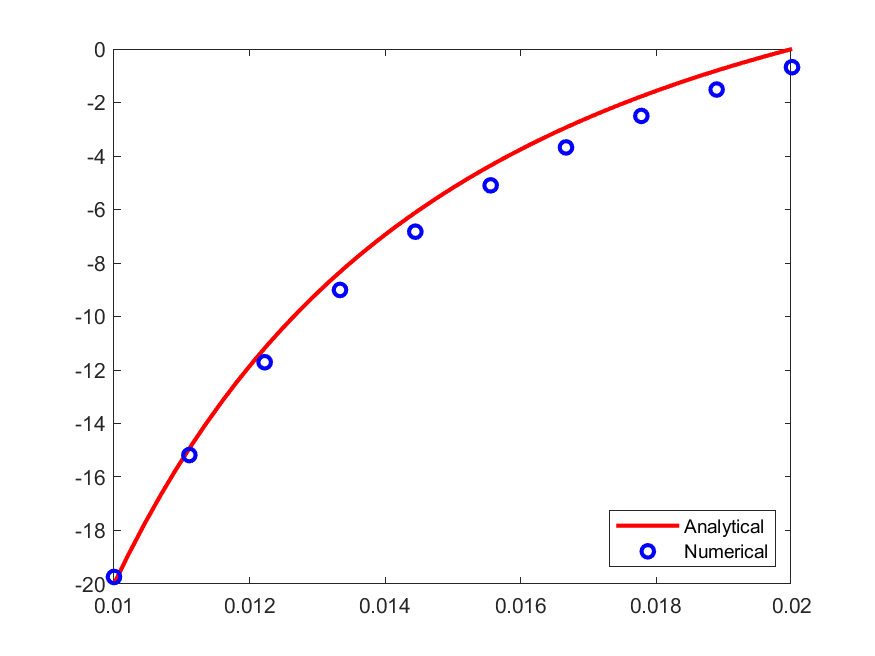
\includegraphics[width=95mm]{graphs/SigmaR.png}
\caption{Зависимость радиальных напряжений от радиуса}
\label{1r}
\end{center}
\end{figure}


\begin{figure}[h]
\begin{center}
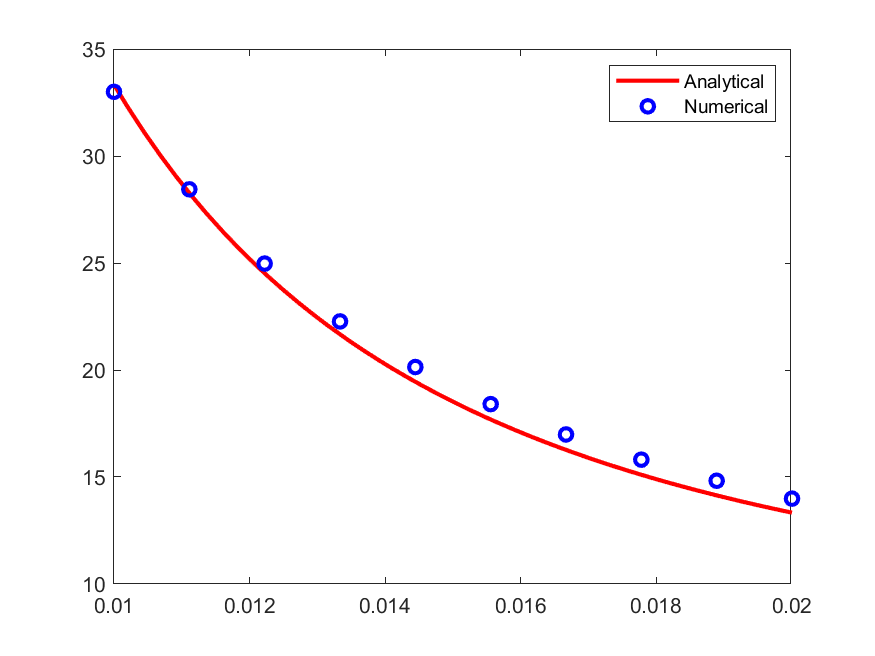
\includegraphics[width=95mm]{graphs/SigmaT.png}
\caption{Зависимость окружных напряжений от радиуса}
\label{1t}
\end{center}
\end{figure}
Расчёт относительной погрешности для следующей таблицы был произведён по формуле :
\begin{equation}\label{Error_Ot_L2}
\sqrt{\sum_{i=1}^{n} \dfrac{ (u_i^{an}-u_i^{me})^2}{ (u_i^{an})^2 }}
\end{equation}
где $u^{an}$ - аналитическое решение, $u^{me}$ - численное решение. Не было использовано выражение $\dfrac{s_{i}}{\sum{s_i}}$, в следующем расчёте будет добавлен данный множитель. Для сетки N=200 при количестве подобластей $Coef_Overlapping=10$ расчёт не получился по непонятным причинам. Буду разбираться с этой проблемой. 

\begin{table}
\caption{Относительная погрешность для разных сеток, пространство $L_2$}
\begin{tabular}{|l|c|c|c|}\hline
\diagbox[width=10em]{Кол-во\\подобластей}{Сетка}&
  50 & 100 & 200 \\ \hline
1 & 2.72$\times 10^{-2}$ & 1.36$\times 10^{-2}$ & 6.78$\times 10^{-3}$ \\ \hline	
2 & 2.65$\times 10^{-2}$ & 1.33$\times 10^{-2}$ & 6.61$\times 10^{-3}$ \\ \hline
4 & 2.53$\times 10^{-2}$ & 1.21$\times 10^{-2}$ & 5.57$\times 10^{-3}$ \\ \hline
10 & 1.62$\times 10^{-2}$ & 1.05$\times 10^{-2}$ & ERROR \\ \hline
\end{tabular}
\end{table}

\newpage
\begin{comment}
\begin{table}[h]
\caption{Нормы ошибок для $C_{1}$}
\label{tabl:2}
\begin{center}
\begin{tabular}{|p{6em}|p{2.5em}|p{7em}|p{7em}|p{7em}|}
\hline
Метод \newline конечных элементов &h, мм & относительная погрешность перемещений, м & относительная погрешность радиальных напряжений, МПа &  относительная погрешность окружных напряжений, МПа \\
\hline
\multirow{3}{*}{Стандартный}
& 0.02 & 7.96$\times 10^{-5}$ & 2.63$\times 10^{-2}$ & 1.57$\times 10^{-2}$ \\ \cline{2-5}
& 0.01 & 1.99$\times 10^{-5}$ & 1.32$\times 10^{-2}$ & 7.93$\times 10^{-3}$ \\ \cline{2-5}
& 0.005& 4.97$\times 10^{-6}$ & 6.64$\times 10^{-3}$ & 3.98$\times 10^{-3}$ \\ \hline
\multicolumn{5}{|c|}{}\\
\hline
\multirow{3}{*}{Смешанный}
&0.02 & 2.57$\times 10^{-5}$& 2.62$\times 10^{-2}$ & 1.57$\times 10^{-2}$ \\ \cline{2-5}
&0.01 & 6.43$\times 10^{-6}$& 1.32$\times 10^{-2}$ & 7.92$\times 10^{-3}$ \\ \cline{2-5}
&0.005& 1.61$\times 10^{-6}$& 6.64$\times 10^{-3}$ & 3.98$\times 10^{-3}$ \\ \hline
\end{tabular}
\end{center}
\end{table}

\begin{table}[h]
\caption{Отношение норм ошибок для $C_{1}$}
\label{tabl:2ot}
\begin{center}
\begin{tabular}{|p{6em}|p{6.5em}|p{4em}|p{4em}|p{4em}|}
\hline
Метод \newline конечных элементов& отношение \text{шагов по} пространству &отнош. погрешностей u & отнош. погрешностей $\sigma_{rr}$ & отнош. погрешностей $\sigma_{\varphi\varphi}$ \\ 
\hline
\multirow{2}{*}{Стандартный}
&0.02/0.01=2  & 4  & 1.99 & 1.98 \\ \cline{2-5}
&0.02/0.005=4 & 16 & 3.96 & 3.95 \\ \hline
\multicolumn{5}{|c|}{}\\
\hline
\multirow{2}{*}{Смешанный}
&0.02/0.01=2  & 4  & 1.98 & 1.98 \\ \cline{2-5}
&0.02/0.005=4 & 16 & 3.95 & 3.94 \\ \hline
\end{tabular}
\end{center}
\end{table}

\newpage

\begin{table}
\caption{Вычисление $\varepsilon^{*}_V$}
\label{tabl:EpsV1}
\begin{center}
\begin{tabular}{|c|c|c|}
\hline
Тип МКЭ & Минимальное значение & Максимальное значение \\
\hline
Стандартный & 0.04663 & 0.1828 \\
\hline
Смешанный & 0.04663 &  0.1828 \\
\hline
\end{tabular}
\end{center}
\end{table}
 
\begin{table}
\caption{Время решения задачи}
\label{tabl:Time1}
\begin{center}
\begin{tabular}{|c|c|c|}
\hline
h & Стандартный МКЭ & Смешанный МКЭ \\
\hline
0.02 & 0.000116749 & 0.006622 \\
\hline
0.01 & 0.0001466 &  0.02458 \\
\hline
0.005 & 0.0003759 &  0.222698 \\
\hline
\end{tabular}
\end{center}
\end{table}
\end{spacing}


Анализ полученных результатов показал, что:
\begin{itemize}
\item[-]полученные двумя методами радиальные и окружные напряжения достаточно близки друг к другу;
\item[-]для напряжений наблюдается линейная скорость сходимости численного решения к аналитическому при измельчении сетки, для перемещений - квадратичная;
\item[-]при использовании смешанного метода конечных элементов существенно возрастают вычислительные затраты по сравнению с использованием стандартного метода конечных элементов;
\end{itemize}

Отметим, что значения радиальных напряжений на внутренней и внешней поверхностях трубы, полученные смешанным и стандартным методами конечных элементов, соответствуют приложенным давлениям. 

На рисунках \ref{1r}-\ref{1t} показаны распределения напряжений для сетки с шагом h=0.01 (N=100). Синим обозначено аналитическое решение, красным квадратом -численное решение, полученное стандартным методом конечных элементов, чёрным ромбом- численное решение, полученное смешанным методом конечных элементов. 

\newpage
\begin{figure}[h]
\begin{center}
\includegraphics[width=70mm]{ELR1_2.png}
\caption{Зависимость радиальных напряжений от радиуса}
\label{1r}
\end{center}
\end{figure}

\begin{figure}[h]
\begin{center}
\includegraphics[width=80mm]{ELT1_2.png}
\caption{Зависимость окружных напряжений от радиуса}
\label{1t}
\end{center}
\end{figure}

\newpage

\begin{center}
\section*{\centering ЗАКЛЮЧЕНИЕ}
\end{center}
\addcontentsline{toc}{section}{ЗАКЛЮЧЕНИЕ}

Цели и задачи, поставленные в бакалаврской работе, выполнены. Изучены математические модели для краевой задачи упругости и краевой задачи с учётом деформации ползучести, исследованы стандартный и смешанный методы конечных элементов для численного решения поставленной задачи. Данные методы реализованы в виде программы, написанной на языке $C++$. Проведены серии расчётов для задачи нагружения упругой трубы давлением. Выполнено тестирование программы путём сравнения численных решений с аналитическим решением рассмотренной задачи, проведено сопоставление численных решений, полученных стандартным и смешанным методами конечных элементов. 

Проведённый анализ норм ошибок для краевой задачи упругости показал, что для расчёта перемещений получен второй порядок точности, а для напряжений - первый порядок. Сравнение результатов при разных коэффициентах Пуассона показало, что для слабосжимаемого материала правильнее использовать смешанный метод конечных элементов, так как ошибки в вычислении напряжений при решении стандартным методом конечных элементов существенно возрастают, в то время как смешанный метод конечных элементов обладает стабильной точностью.

Проведённый анализ норм ошибок для краевой задачи с учётом деформации ползучести показал, что смешанный метод конечных элементов эффективнее стандартного метода конечных элементов, так как с течением времени аналитическое и численное решения начинают расходиться. Чем мельче сетка, тем медленнее происходит рост ошибки. Для смешанного метода ошибка увеличивается значительно медленнее, чем при использовании стандартного метода.

\end{comment}

\end{document}

